\chapter{Experiments}

\section{Experimental Protocols}
\subsection{Bacteria culture}

Experiments were done with the non-chemotactic, smooth swimmer strain of \textit{E.coli} JEK1038 (W3110 [lacZY::GFPmut2, cheY::frt], green) provided by prof.\ Juan Keymer. The strain was modified to express the green fluorescent protein GFPmut2, and its run-and-tumble dynamics were suppressed by cheY deletion \cite{VanVliet2014ThePopulations}. 

Bacteria stocks are stored at \SI{-20}{\degreeCelsius}. To initiate a new bacterial culture, \SI{20}{\micro\liter} are put in \SI{5}{\milli\liter} of Lysogeny Broth (LB) medium for approximately 24 hours in an incubator with a shaker at \SI{28}{\degreeCelsius} and \SI{180}{\rpm}. Then, \SI{30}{\micro\liter} of this overnight were diluted in \SI{3}{\milli\liter} of LB medium with \SI{3}{\milli\molar} isopropyl $\beta$-D-1-thiogalactopyranoside (IPTG Sigma-Aldrich) and grown until the optical density at \SI{600}{\nano\meter} (\SI{}{\OD}) reaches $0.5\pm0.05$. Afterward, we added $0.1\%$ w/v bovine serum albumin (BSA) to avoid cell-to-cell adhesion and centrifuge the culture for $15$ minutes at \SI{4600}{\rpm} or $2600$ relative centrifugal force (rcf), leaving a bacteria pellet at the bottom of the falcon tube. We resuspended the pellet in \SI{3}{\milli\liter} of MMA, resulting in a mixture with an \SI{}{\OD} slightly lower than $0.5$. MMA or minimal motily media is a phospate buffer where bacteria can live, but prevents cell division \cite{Altshuler2013Flow-controlledConstriction}. MMA is composed of \SI{10}{\milli\molar} K$_2$HPO$_4$, \SI{10}{\milli\molar} KH$_2$PO$_4$, \SI{0.1}{\milli\molar} EDTA and \SI{20}{\micro\molar} sodium lactate. To reach a low bacterial density, we again diluted until \SI{5d-4}{\OD} is reached. It is important to mention that \SI{}{\OD} is insufficient to determine the final density in our experiments since bacteria will not enter the channel evenly every time because they move through the walls. We assume that these density variations are sufficiently small not to affect the dynamics of each regime.


\subsection{Fabrication of microfluidic devices}

\begin{figure}[H]
	\centering
	\includesvg[scale=1]{imagenes/channel diagram}
	\caption[Channel diagram]{Diagram of the 3D perspective of the channel for one amplitude $A$ and different wavelength $\lambda$, not at scale. The frontal side of this sketch will face towards the microscope slide after forming the PDMS-PDMS bonds. For each channel, the curved wall has a sinusoidal form with one amplitude $A$ and different wavelengths $\lambda$. There are four different channels with amplitudes $A=$ \SIlist[list-units=single, list-final-separator = {, }]{3;6;9;12}{\micro\meter} and each one is divided into four sections with wavelengths $\lambda=$ \SIlist[list-units=single, list-final-separator = {, }]{21;24;27;30}{\micro\meter} allowing to study in a range of curvatures.}
	\label{channel_diagram}
\end{figure}

In the experiments, we put the bacteria suspension in a microfluidic channel that is \SI{100}{\micro\meter} width and \SI{25}{\micro\meter} deep and have three flat walls and one curved in a sinusoidal form. The channel is divided in several sections with different combinations of amplitudes $A$ and wavelengths $\lambda$. Figure \ref{channel_diagram} shows a diagram of the channel.  The nominal values of the amplitudes are  $A=$ \SIlist[list-units=single, list-final-separator = {, }]{3;6;9;12}{\micro\meter} and the wavelengths $\lambda=$ \SIlist[list-units=single, list-final-separator = {, }]{21;24;27;30}{\micro\meter}. 


We fabricated the microfluidic devices with conventional optical lithography techniques to create a mold with the shape of the channels. The mold creation process begins with cleaning a silicon wafer in the plasma cleaner for 8 minutes. The objective is to remove organic contaminants and dehydrate the substrate. Then the photoresist (SU-8) is added, approximately up to half the diameter of the wafer. The wafer is rotated in a spin-coater, first at \SI{500}{\rpm} for \SI{60}{\second} to distribute the photoresist over the entire surface of the wafer, and then by the final rotation speed \SI{3100}{\rpm} for \SI{40}{\second}, to reach the desired thickness of \SI{25}{\miro\meter}. The higher the rotation speed, the thinner the film left on the wafer. The next step is to evaporate the solvent from the resin so that a dry layer remains. This is done on a hotplate in two steps, the first at \SI{65}{\degreeCelsius} for 15 minutes, the second at \SI{95}{\degreeCelsius} for 35 minutes. The design is printed on this film, using a maskless laser writer that draws with a UV laser the design on the wafer coated with SU-8. This is a negative resin, which means that everything that is exposed to UV light will reticulate and remain on the wafer after development. This happens because the UV light interacts with the salt in the solution creating hexafluoroantimonic acid that then protonates the epoxides groups in the resin monomers. The monomer are thus activated but the polymerization will not proceed significantly until the temperature is raised as part of the post expose bake. The post-bake heating process is also divided in two parts of \SI{65}{\degreeCelsius} for 15 minutes and \SI{95}{\degreeCelsius} for 40 minutes. Here the formed polymers will cross-link, meaning that they will form bonds that link one polymer chain to another. After baking the wafer, it is developed, i.e. it is immersed in propylene glycol monomethyl ether acetate (PGMEA) for 3 minutes until all unexposed resin is dissolved and then the wafer is washed with isopropanol. Finally the wafer is baked at \SI{135}{\degreeCelsius} for 2 hours to increase the crosslinking rate inducing elimination of cracks or unstuck parts. At the end of the process the wafer has a pattern with the shape of the channels.

The UV laser does not focus perfectly so the real values of the amplitude and wavelength differ from the nominal values, mostly on the amplitude $A\sim$ \SI{12}{\micro\meter} where the differences are up to \SI{2}{\micro\meter}. Nevertheless, both $A$ and $\lambda$ were measured for every channel section. The measured dimensions will be used to characterize channels. 

The wafer is put in a petri dish and filled with polydimethylsiloxane (PDMS). We prepare a PDMS mixture of Sylgard 184 elastomer (Dow Corning) base and curing agent in a 10:1 mass ratio. It is essential to mix for several seconds to ensure the PDMS is homogenous. If the mixing is not enough, some parts of the PDMS might not separate from the mold and cause irregularities on the channel. Then, the mixture should be centrifuged for 10 minutes at 5000 rpm to degas it. To ensure there is no air after pouring the mixture on the mold, it is necessary to put the mold in a vacuum chamber. The remaining bubbles will expand and merge, so they pop more easily. Finally, the mold is left in an oven at \SI{65}{\degreeCelsius} for at least $1$ hour. If the air bubbles were not removed, they would expand during the heating process and could ruin the shape of the channel. After removing each channel from the mold, we made two entrance pools at opposite ends of the channels with a \SI{4}{\milli\meter} tissue punch for each channel.

We also considered that the channel must have the four walls made of PDMS to avoid different mechanical or chemical properties on the walls. To do so, we cover a microscope slide with a thin layer of $\sim$ \SI{0.4}{\gram} of PDMS, spread with a plastic spatula. The slide is left overnight on top of a leveled surface, so PDMS uniformly distributes, and then it is put into the oven. Using a plasma cleaner, it is possible to bond the channel with the slide \cite{Henry2015ScholarlyCommonsProtocol-Technics}. We set the RF level to maximum power and exposed the PDMS block with the microchannel and the PDMS-covered glass to air plasma for 1 minute. PDMS is comprised of repeated units of -O-Si(CH$_3$)$_2$. The exposure to an oxygen plasma will form silanol groups Si-OH, so when a similar surface is brought into contact, covalent Si-O-Si bonds are created, displacing a water molecule \cite{Koh2012QuantitativeEffect}. Finally, plasma oxidation will make the channel surface hydrophilic. The final assembly is shown in the figure \ref{experimental_setup} a). 

\begin{figure}[H]
	\centering
	\includesvg[scale=1]{imagenes/experimental_setup}
	\caption[Microfluidic device diagram]{a) Diagram of the empty microfluidic device. The red line is the channel where all the experiments are performed. b) Diagram of the microfluidic device when the bacteria suspension is added. The bacteria suspension, represented as green, fills both pools and the channel.}
	\label{experimental_setup}
\end{figure}

\subsection{Experimental setup}

\begin{wrapfigure}{r}{0.5\linewidth}
% \vspace{-50pt}
\centering
\includesvg[width=\linewidth]{imagenes/focal plane}
\caption[Focal plane diagram]{Diagram of the focal plane, shown in red. The depth of the focal plane is \SI{2}{\micro\meter} so the depth of the channel does not matter in the observed dynamics. }
% \vspace{-50pt}
\label{focal_plane}
\end{wrapfigure}

Since \textit{E.coli} cell membrane is negatively charged, adsorption of cells to walls might occur. We coated the channel walls with $0.1\%$ BSA solution dissolved in MMA to prevent it. BSA also has negative charges so that it will act as a blocking protein. Then, we add bacteria and seal the access holes with a glass coverslip preventing external flows in the experiment, as shown in figure \ref{experimental_setup} b). We used an inverted microscope (Nikon TS100F) with a 40x/0.6 NA Plan Fluor objective to measure bacteria fluorescence and recorded it with a camera (Andor Zyla 2048 × 2048 \SI{}{\square\pixels}) at 10 fps, gain $4$, and 2x2 binning giving a resolution of \SI[per-mode = symbol]{0.32}{\micro\meter\per\pixels}. Since the PDMS thickness may vary, adjusting the correction ring of the objective to the appropriate dimensions is necessary. The focal plane will be on the edge of the channel, whose depth is approximately \SI{2}{\micro\meter}. Therefore we assume that the depth of the channel (\SI{25}{\micro\meter}) will not affect the observed dynamics. Figure \ref{focal_plane} shows a diagram of the focal plane. 


\section{Image analysis}


This section describes how we analyzed the videos obtained from the experiments. A video can be considered as a 3-axis matrix with values $v_{ij}^t$ where $i,j$ are the pixel position indices and $t$ represents the frame number. The value of $v_{ij}^t$ is the intensity of that pixel. The measured intensities have two sources, camera noise $n_{ij}^t$ and bacteria fluorescence $b_{ij}^t$. Our goal is to use $b_{ij}^t$ to measure different properties of the system. In figure \ref{video_histogram} it is possible to see a typical frame and histogram for the intensities $v_{ij}^t$.

\begin{figure}[H]
	\centering
	\includesvg[scale=1]{imagenes/typical_video_frame}
	\caption[Typical video frame]{a) Example of one frame in a video and b) probability density function (pdf) of the intensity for the entire video. The video is saved in a 12-bit format so the intensities for each pixel $v$ can take values from $0$ to $4096$. }
	\label{video_histogram}
\end{figure}

\subsection{Mask creation}

Masks are binarized images that determine the region of interest (ROI) for the experiment. In this case,  we look for the region where bacteria swim, bounded by the flat and sinusoidal walls. The procedure starts by creating an image $W$ from the original video that contains the maximum value reached for each pixel in the video $W_{ij}={\rm max}_{t\in[1,T_{max}]} v_{ij}^t$. Pixels that only represent noise will have maximum values $W_{ij}$ around the noise distribution, but the presence of a bacterium in a pixel at a given time will considerably increase the obtained maximum value at that pixel. Since bacteria mostly swim near walls, we can measure the contour of the walls as we see in figure \ref{mask} a). In order to binarize the image, we use the OpenCV python package whose thresholding function includes Otsu's binarization algorithm \cite{Grdiet2013BinarizationABSTARCT}. This method will automatically calculate a threshold for the image as a point between two intensity peaks. As we see in figure \ref{mask} b), the histogram has optimal conditions for this method. By doing this, we can detect the wall boundaries, and by filling all the pixels in between with ones, we can create a binary image with the region of interest as shown in figure \ref{mask} c). Finally, the tilting angle of the experiment can be measured as the angle between the x-axis and the flat wall. Thus the binarized image and the whole video can be rotated to produce a horizontal wall. The final result is displayed in figure \ref{mask} d). 

\begin{figure}[H]
	\centering
	\includesvg[scale=1]{imagenes/mask_example}
	\caption[Mask example]{a) Max pixel intensity image, created directly from the video. b) Pdf of the max pixel intensity image $W$. The first peak of the histogram is associated with the noise distribution $n_{ij}^t$ and the second with $b_{ij}^t$. c) Binary mask derived from the max intensity image and d) the rotated mask, so the flat wall is horizontal. }
	\label{mask}
\end{figure}

\begin{wrapfigure}{r}{0.5\linewidth}
\vspace{-20pt}
\centering
\includesvg[width=\linewidth,angle=0]{imagenes/bands}
\caption[Bands example]{Image of the bands for the same mask shown in figure \ref{mask} c).}
\label{bands}
\end{wrapfigure}


The mask serves two primary purposes. The first one is to determine the actual dimensions of the channel. We manually enter the position of the peaks and valleys to the program. The amplitude $A$ is half of the mean vertical distance between a peak and a valley from the input locations, while the wavelength $\lambda$ is the horizontal separation between two consecutive peaks or valleys. The input has subpixel precision, so errors are only associated with mouse movement. Errors are not systematic because they are added randomly, so the method gives reasonable measures.  An automatic version will introduce many problems, as the border of the mask is not smooth, making many criteria not robust.

The second purpose is to define the boundary of the experiment. We define the bands $B_{c},B_{f}$ around the curved and flat walls respectively, to be \SI{4}{\micro\meter} thick from each wall into the bulk system. Bands are used to measure the density near walls and to decide if a bacterium is in contact with the wall or not. In figure \ref{bands} there is an example showing both bands. The width of the bands was chosen to ensure that bacteria swimming in contact with the wall fall entirely inside the band region. In some cases, bacteria will be swimming barely not in contact with the wall but still inside the band region. These cases are considered marginal since most of them will reach the wall one or two frames later.


\label{section: noise remove}
\subsection{Noise treatment}

\afterpage{%
\begin{figure}[H]
	\centering
	\includesvg[scale=1]{imagenes/noise_example}
	\caption[Mean noise example]{ a) Mean noise image obtained averaging over time $N_{ij}^t$. The experiment displayed is one where the noise inhomogenities are clearly seen. b) Pdf of $N_{ij}^t$ over two $20 \times 500$ \SI{}{\square\pixels} windows, one in PDMS and the other on MMA. The noise distribution on MMA is shifted to the right compared with the one on PDMS. Also, the difference is greater toward higher values, probably due to the influence of bacteria out of the focal plane. c) Pdf of $N_{ij}^t$ only for pixels in the ROI, where the dashed black line is on $N=n_{\text{est}}$. The ${\rm mean_{ROI}}$ function calculates the mean over this distribution. d) Histogram of $B_{ij}^t$, the video that is used for future measurements. The dashed black line is on $B=0$.  }
	\label{noise_img}
\end{figure}
}

As we said, the intensity values are given by $v_{ij}^t  = n_{ij}^t +  b_{ij}^t$. We are only interested in $b_{ij}^t$, and therefore, we want to minimize the effects of the noise. One important thing to consider is that the mean noise intensity is not the same for every pixel. In other words, the probability density function of noise intensities depends on space. There are two main reasons for this inhomogeneity. First, there are different noise levels at the PDMS and the MMA because out of focus bacteria contribute to the noise, and we can see in figure \ref{noise_img} a) and b) that the noise is higher on the liquid. Second, the illumination is inhomogeneous because we close the diaphragm to decrease noise intensity, only allowing light in the ROI to enter the camera, but the effect is more intense on the edges of the image. This effect is often less important than the first.

To deal with the space dependence of $n_{ij}^t$, we exploit many properties of the data. We first approximate the noise distribution by just calculating the mean intensity of  $\bar{v} = \langle v_{ij}^t \rangle_{ijt}$ where the average is over space and time, as the lower indices indicate. Since for most pixels, the bacteria intensity $b_{ij}^t=0$ as bacteria occupy a small fraction of the ROI, $\bar{v}$ is slightly greater than the mean of $n_{ij}^t$ for different pixels. Now, we assume that every pixel satisfying $v_{ij}^t  < \bar{v} + 3 \sigma$ where $\sigma$ is the standard deviation of $v_{ij}^t$ do not include bacteria fluorescence, i.e. $b_{ij}^t =0$. The $v_{ij}^t$ values that satisfy the previous inequality are renamed as $N_{ij}^t$ because they represent an approximation of the noise. Then, we are only interested in the region with MMA and bacteria, so we estimate the mean of the noise in that region:

\begin{equation} \label{eq:noise_aproximation}
	n_{\text{est}} \equiv {\rm mean_{ROI}}(N_{ij}^t).
\end{equation}

Here the ${\rm mean_{ROI}}$ function represents the mean in time and space of the values of $N_{ij}^t$ for pixels in any frame but inside the ROI defined by the mask. The pdf of $N_{ij}^t$ in the ROI is shown in figure \ref{noise_img} c). The resulting $n_{\text{est}}$ is then substracted to the video so now the intensities on the video are given by $B_{ij}^t  =  v_{ij}^t - n_{\text{est}} =  b_{ij}^t + \tilde{n}_{ij}^t$, where $\tilde{n}_{ij}^t  \equiv n_{ij}^t - n_{\text{est}}$. The pdf of $B_{ij}^t$ is shown in figure \ref{noise_img} d). We observe that the mean of the noise distribution is now close to zero, meaning that the matrix $\tilde{n}_{ij}^t$ averages 0 in the ROI. Now the matrix $B_{ij}^t$ has negative values, so it is not a measure of the intensity of bacteria as it is strictly positive. Nevertheless, due to the subtraction of the average noise, an average in time and space of $B_{ij}^t$ only has contributions from $b_{ij}^t$. Since bacteria intensity is proportional to density, the average of $B_{ij}^t$ is and indirect measurement of mean bacterial density.

\subsection{Intensity analysis}

The properties of the $B_{ij}^t$ matrix give the possibility to measure mean bacteria intensity over time and space identically as measured with $ b_{ij}^t$. We are interested in how bacteria behave in the bands of each wall and how both walls compare. We begin by considering $M_{ij} = \langle B_{ij}^t \rangle_t $. The image $M_{ij}$ is called the mean image of the experiment and is an indicator of where bacteria swam through. An example of $M_{ij}$ is shown in figure \ref{mean_image_and_profile} a). The curved wall has a sinusoidal form, so it is reasonable to average $M_{ij}$ over every period. If the experimental data of one video has $N_{\text{exp}}$ periods, the average intensity in one period $D_{xj}$ is given by:

\afterpage{
\begin{figure}[H]
	\centering
	\includesvg[scale=1]{imagenes/mean_image_and_profile}
	\caption[Mean image and profile of an experiment]{Mean image and profile of an experiment with $A=$ \SI{5.7}{\micro\meter} and $\lambda = $ \SI{30}{\micro\meter}. a) Mean image $M_{ij}$ of a experiment where pixels outside of the ROI where colored in black. The accumulation on the walls can be seen. b) Mean intensity over a period for the mean image shown in a). Both images share the same colorbar. c) Normalized intensity $I(x)$ for all experiments that share dimensions with the mean image of a). The profile of the flat wall fluctuates around 1 for all experiments and will be omitted from now on. The errorbars are the $95\%$ confidence interval of the mean $I(x)$ over the $N$ periods.}
	\label{mean_image_and_profile}
\end{figure}
}

\begin{equation} \label{eq:2d density}
	D_{xj} = \frac{1}{N_{\text{exp}}} \sum_{n=1}^{N_{\text{exp}}} M_{x+ n\lambda,j}.
\end{equation}

The matrix $D_{xj}$ is an indirect measurment of the mean two-dimensional density in one period of the curved wall. We use the coordinate $x$ instead of $i$ to emphasize that $x$ only takes values among one wavelength as the average is on every period. The position of the valley corresponds to $x=0$. Figure \ref{mean_image_and_profile} b) shows an example of $D_{xj}$. Then we consider the intensity near a wall $i_i^w$ as:

\begin{equation}
	i_x^w = \sum_{j \in B_w} D_{xj},
\end{equation}

where $B_w$ is the band of a specific wall $w$, meaning that $w$ is either $c$ or $f$ depending if the wall is curved of flat respectively. Then the definition of $i_x^w$ is the vertical sum of $D_{xj}$ over the band $B_w$. We normalize the intensity profiles by the mean of the flat wall intensity profile $\bar{i}^f = \langle  i_x^f\rangle_x $. 

\begin{equation}  \label{eq:Intensity profile on experiment}
	I_{\text{exp}}^w(x) = \frac{i_x^w}{\bar{i}^w}.
\end{equation}

With this definition the normalized profile of the flat wall shows little fluctuations around $1$ for all experiments. The flat wall profile may have inhomogenities if a bacteria is adhered to the surface, but that never happens if the channel is coated with BSA. Therefore, the flat wall profile carries no relevant information for the analysis. For simplicity, from now on we define $I_{\text{exp}}(x)$ as the normalized intensity profile of the curved wall, without the upper index $c$. Here we maintain the label $\text{exp}$ to remember that this is the result from the video of one experiment. The normalization allows the comparison between different experiments respect to the standard of the flat wall. Therefore it is possible to define the mean normalized intensity profile $I(x)$ as the weigthed average of the $I_{\text{exp}}(x)$ profiles of experiments that share the same amplitude $A$ and wavelength $\lambda$. If $\mathbb{E}_{A,\lambda}$ is the set of experiments that share the same values of $A$ and $\lambda$, we calculate $I(x)$ as:
 
 \begin{align}
    N &= \sum_{\text{exp} \in \mathbb{E}_{A,\lambda}} N_{\text{exp}},     \\
    I(x) &= \sum_{\text{exp} \in \mathbb{E}_{A,\lambda}} I_{\text{exp}}(x) \frac{N_{\text{exp}}}{N},
    \label{eq:Intensity profile}
 \end{align}
 
where $N$ is the total number of periods considered in the average. One set of profiles is displayed in figure \ref{mean_image_and_profile} c) as an example. When $I(x)$ is lower than 1, the intensity is lower in the curved wall than in the flat wall. We interpret this as a lower concentration of bacteria in the curved wall as compared to the flat one. The values of $A$ and $\lambda$ will be specified in all figures with an intensity profile. Chapter 4 will profoundly discuss all the information and physics related to intensity profiles.


\subsection{Bacteria tracking}


Tracking, in general, refers to determining the trajectories of objects in an image sequence. There are two main steps when doing the tracking: object detection and track creation. In this subsection, we will describe two different methods for doing detection and the tracking method based on linear assignment problems (LAP tracker). These methods are the ones that were the most succesful during this MSc thesis, but other options were studied as well. All of the methods that will be discussed are already implemented on Trackmate, an open-source plugin for Fiji \cite{Tinevez2017TrackMate:Tracking}. 


We start by describing object detection. The specific objective is to determine bacteria position via the intensity $B_{ij}^t$. Then, a detection algorithm should be able to measure intensity variations indicative of the presence of bacteria. One possibility is to use the Laplacian of Gaussian detector (LoG) \cite{Kong2013AApplications,Sage2005AutomaticDynamics}. This method is easier to understand if the matrix $B_{ij}^t$ is thought of as a scalar field $B(x,y,t)$. We only know the field values at a regular grid of point, but we can calculate integrals and derivatives using standard numerical methods. As the detector's name indicates, we first convolve with a Gaussian and then calculate the Laplacian of the result. The equations for the method are:  

\begin{align}
	G(x,y;\sigma) &= \frac{1}{\sqrt{2\pi \sigma^2}} \exp\left(  -\frac{x^2+y^2}{2\sigma^2} \right), \\
	B^{gb}(x,y,t;\sigma) &= B(x,y,t) * G(x,y;\sigma), \\
	R(x,y,t;\sigma)  &= \nabla^2 B^{gb}(x,y,t;\sigma). \label{LoG:result}
\end{align}

Here $G(x,y;\sigma)$ is a Gaussian kernel that, when convolved ($*$ operation) with the image, produces a smoothed version $B^{gb}(x,y,t;\sigma)$ where $gb$ stands for gaussian-blurred. The reason for the smoothing effect of this convolution is that it acts as a low-pass filter for the field \cite{WaltzaAnMachines}, removing highly space-dependent noise contributions. The value of $\sigma$ is $r/\sqrt{2}$ where $r$ is the estimated bacteria radius. More importantly, in equation \eqref{LoG:result} the Laplace operator $\nabla^2$ is applied to $B^{gb}(x,y,t;\sigma)$ to obtain $R(x,y,t;\sigma)$. The result is that bacteria with maximum intensity in the center will also have a minimum negative Laplacian there, so local minima in $R(x,y,t;\sigma)$ are bacteria centers. Locality, in this case, refers to a circle of the estimated radius $r$, so the method detects bacteria as blobs of that size. There are more generalized versions of LoG that allowfor non-circular particles \cite{Kong2013AApplications}. This method is ideal for images with noise and particles with a maximum intensity at their center and decaying at a radius $r$, but it only detects circumferences, so it should not be used if it is necessary to know the exact shape of the particles or their orientations.

\begin{wrapfigure}{r}{0.5\linewidth}

\centering
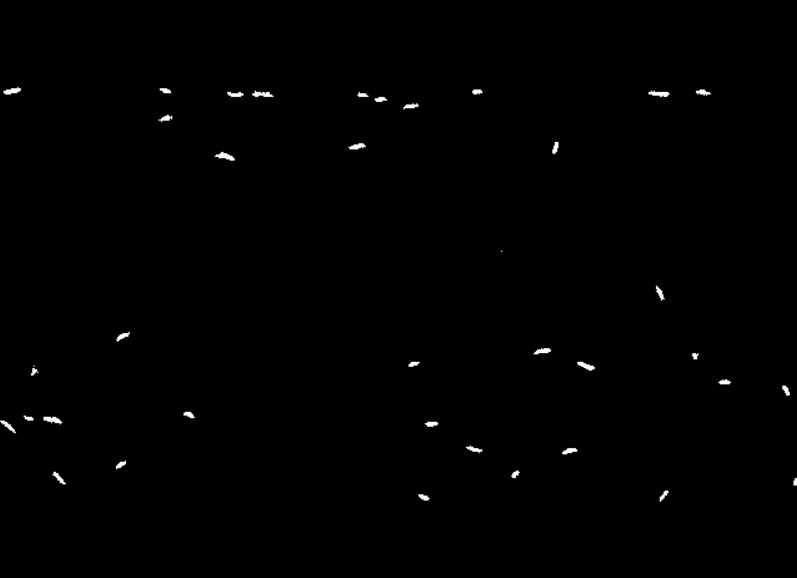
\includegraphics[width=\linewidth,angle=0]{imagenes/track_video_frame.PNG}
\caption[Tracking video frame]{Example of a typical frame for the binarized matrix $T_{ij}^t$.}
\label{tracking_video_frame}
\vspace{-20pt}
\end{wrapfigure}

Another possibility to consider is binarizing the videos. A binarized image will have sharp variations of intensity, and if done correctly, will not lose bacteria in the process. In our case, we again use Otsu's binarization method into the matrix $B_{ij}^t$. The result is then used for the tracking, so we call it $T_{ij}^t$. An example of a typical frame of this tracking video is shown in figure \ref{tracking_video_frame}. Bacteria detection in  $T_{ij}^t$ as simple as considering all connected regions as a particle. This detection method is known as the thresholding detector. One possible issue is that there is only one detection when multiple cells collide. In figure \ref{detection_method_comparison} there is a comparison with results for the two methods. The LoG detector works well with noise, which does not mean that it will fail with a binarized image. Proper binarization often helps with any detection method. Conversely, the thresholding detector adapts to bacteria form and does not make fake detections. This last point convinced us to use a thresholding detector for these experiments.

\begin{figure}
	\centering
	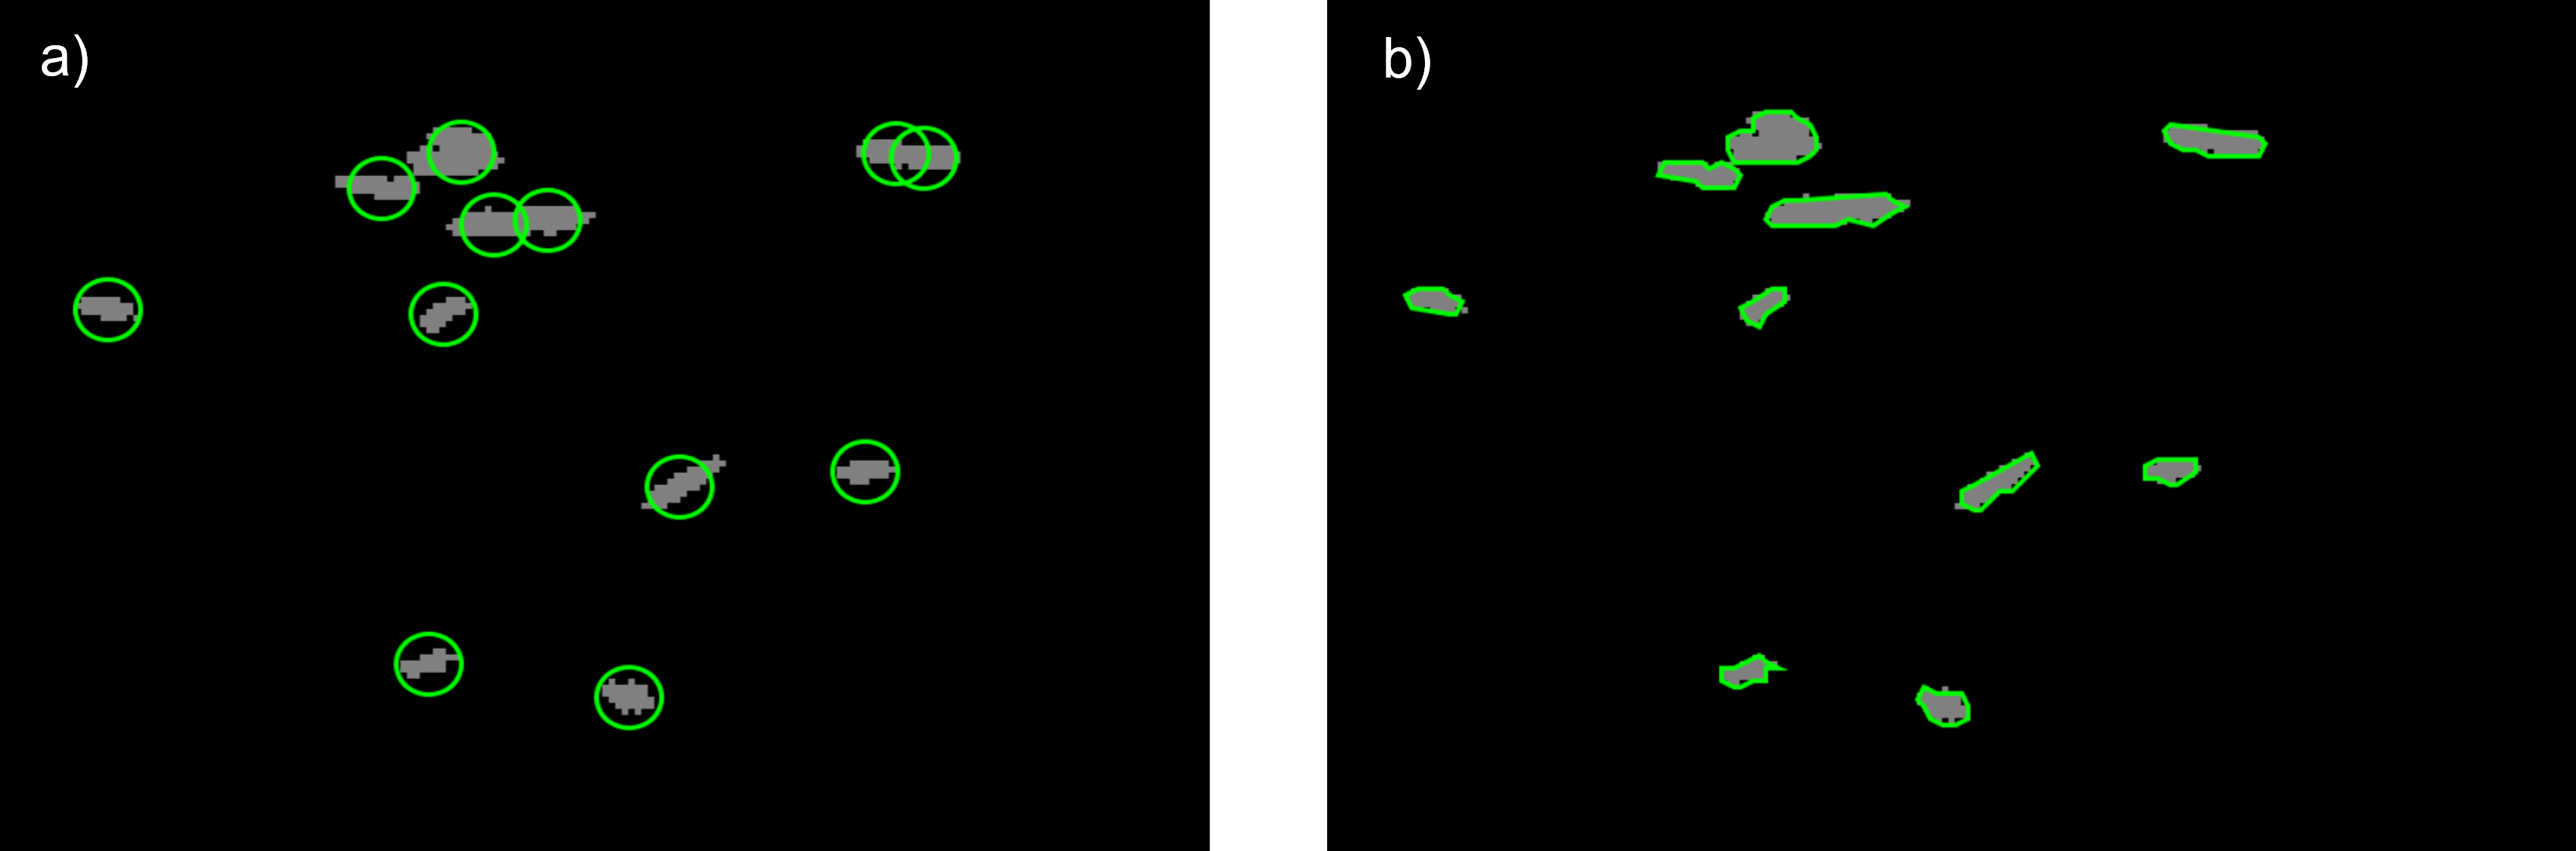
\includegraphics[width=\linewidth]{imagenes/detection_method_comparison.png}
	\caption[Detection method comparison]{ Zoom image of a video $T_{ij}^t$, and bacteria detection results displayed in green for a) LoG detector and b) Thresholding detector. LoG detector adds virtual detections in large bacteria, but the thresholding method will account for multiple bacteria collisions as only one particle. Methods give comparable results, but the best choice will depend on experimental properties, such as bacteria shape and frequency of collisions. In our case, Otsu's binarization method has the conditions to perform the algorithm successfully, so the overall thresholding detector b) has better results than the LoG detector a). }
	\label{detection_method_comparison}
\end{figure}

Now we deepen into the automatic tracking method described in Trackmate's user manual. There are many options for automatic tracking that use simple criteria such as the nearest neighbor assignment or overlapping criteria. It is not meriting to explain these methods as they only work under restricted conditions. Instead, the idea behind LAP trackers gives a general tool for tracking without overcomplications \cite{Jaqaman2008RobustSequences}. A linear assignment problem refers to determining the assignment matrix A that satisfies:

\begin{equation}
  A = {\rm argmin} \left(  \sum_{k,l} A_{kl}C_{kl} \right),
\end{equation}

where $C_{kl}$ is a cost matrix and $A_{kl}$ is a boolean matrix of 1 (link) and 0 (no-link) with the restriction that there is only one link for each row or column. To understand how this problem is used for tracking we need to inspect the cost matrix $C$. The simpler form of $C$ is to consider connections between detections of two frames $t$ and $t+1$. These frames will have $n$ and $m$ detections, respectively. Then $C$ is an $(n+m) \times (n+m)$ with four quadrants. 

\begin{itemize}
	\item The top left quadrant of size $n \times m$ has the cost of linking a detection on frame $t$ to one in $t+1$. The cost is $C_{kl} = (D_{kl}P_{kl})^2$ where $D_{kl}$ is the distance between the detections and $P_{kl} = 1 + \sum_f p_{kl}^f$ where $p_{kl}^f$ is a penalization for differences on the particle feature $f$ given by $p_{kl}^f = W_f \frac{|f_k - f_l|}{f_k + f_l}$, where $f_k$ is the value of the feature $f$ for particle $k$. Features that are useful with the thresholding detector are bacteria perimeter and area. The usage of penalization by features requires these characteristics to be held constant for there to be a connection. The magnitude of the feature penalization $W_f$ regulates the importance of this conservation. If $D_{kl}$ exceeds the double of the mean distance traveled in each frame, $C_{kl}$ is set to infinity
	\item Top right and bottom left quadrants are cost for not linking particles for frame $t$ and $t+1$ respectively. The cost values are set to $c = 1.05 \times {\rm max}(C_{kl})$ where the maximum is only taken on the top left quadrant and does not consider the infinite values.
	\item The bottom right quadrant is an auxiliary matrix in the Munkres and Khum algorithm used to solve the LAP problem \cite{Munkres1957AlgorithmsProblems}.
\end{itemize}

Considering the form of the cost matrix $C_{kl}$, depending on the quadrant of the connections, the assignment matrix $A_{kl}$ will connect detections from one frame to another or start/end tracks. Applying this to all frames will create the trajectories of the particles. A similar LAP can be considered for all the resulting tracks. In this case, the goal is to merge tracks, so the cost matrix includes distances between ends and starts of tracks. The cost is infinite if the end occurs at a time $T$ before the start. This process is called gap closing, as it allows to solve gaps in the tracks caused primarily due to detection failures involved in collisions. If particles separate from each other soon after the collision, this process will fix the errors. If they do not, the involved particles could be interchanged, causing wrong links, so the time $T$ should be kept as low as possible.  The LAP tracker as both frame-to-frame linking and gap closing works for general-purpose tracking, but Brownian motion is the best performing case for this method.

Nevertheless, we used a more specific version of the LAP tracker that considers the trajectories' properties in our experiments. The modification is simple but has profound effects. Based on particle trajectories, a prediction of where spots will be in the next frame is made. Instead of linking detections to each other, detections are linked with predictions based on the previous frame. The Kalman filter, also known as the linear quadratic estimation algorithm, is used to make predictions. Kalman filtering is a world in itself and has applications in robotics, navigation of vehicles,  geophysics, among others \cite{Auger2013IndustrialReview,Aanonsen2009TheReview}. Here we need to know that the Kalman filter considers bacteria's previous velocities to predict the future positions. Predictions allow gap closing differently. If two particles collide, there will only be one detection for two tracks. Then, one prediction will not have a link, but another prediction can be made for the next frame based on the previous. Predictions can fail to link up to $N_f=4$ times before the track is ended. If a track successfully encounters a detection before the $N_f$ failed attempts, the gap is closed. However, the predictions are not registered as intermediate positions, only truly measured detections. This method has two more parameters: the initial search radius $r_i=\SI{15}{\pixels}=\SI{4.8}{\micro\meter}$ and the search radius $r_s=\SI{10}{\pixels}=\SI{3.2}{\micro\meter}$. Both are the maximum allowed distances for frame-to-frame linking, with the difference that $r_i$ is only for new track initiation while $r_s$ is for linking considering predictions. The algorithm is briefly summarized as:

\begin{itemize}
	\item In the first frame, particles are linked to the second frame using standard particle to particle connections. The result is many starting tracks whose initial velocity can be measured, so predictions via Kalman filtering are now possible.
	\item For subsequent frames, the LAP is changed to prediction to particle linking, but the cost matrix structure does not change. New velocity measures will be considered in the Kalman filtering predictions.
	\item If a track fails to connect its prediction to a detection, new predictions will be made for future frames based on the current prediction. If this fails up to $N_f$ times, the track is terminated.
	\item Also, new particles could appear, so if a detection fails to find a track, the next frame, that detection will be considered in a separate LAP for tracking initiation. This LAP will be solved only with particles not in a track and after solving the LAP with predictions. This assigning order means that a track creation cannot cause other tracks to end.
\end{itemize}

The algorithm is successful in gap closing and frame to frame linking, bypassing problems caused by collisions. This affirmation only applies if particles have a roughly constant velocity and the search radius $r_s$ is more than the displacement between successive frames. The second point is important because when bacteria collide with a wall, they may completely stop, so a short $r_s$ may exclude these cases, ending the track. All the results of tracking are left for chapter 4; meanwhile, figure \ref{tracking_examples} shows some trajectory examples. In table \ref{table:image analysis parameters} all the relevant quantities for the methods described in this chapter are summarized.

Tracking gives all the positions of a single bacterium connected in time. We can calculate the velocity of particle $i$ in a frame $t$ as:

\begin{equation} \label{eq tracking velocity}
    \dot{\textbf{r}}_i(t) =  \frac{\textbf{r}_i(t+dt)-\textbf{r}_i(t)}{dt},
\end{equation}

where $dt$ is the time difference between two successive detections in a trajectory, and $\textbf{r}_i$ is the position of the $i$-th bacteria. The time resolution of the video is \SI{0.1}{\second}, but $dt$ can be greater if particles are not detected for a brief time, for example, in the case of collisions. The maximum allowed value for $dt$ is \SI{0.5}{\second}. 

\begin{figure}
	\centering
	\includesvg[scale=1]{imagenes/tracking_trajectories}
	\caption[Example of trajectories]{Example of trajectories obtained with the tracking method. The star represents the start of each track and the triangles the end of them. The mask is used as background to show the walls. Dimensions of the curved wall are shown at the bottom.}
	\label{tracking_examples}
\end{figure}


\begin{table}[!h]
   \centering
    \small
    \caption[Summary of all quantities used in the image analysis]{All the quantities used for the image analysis, with their description and values. Parameters that are discussed but not include in the methods are not included in this table. }
    \begin{tabularx}{\textwidth}{lXl}
    \hline\noalign{\smallskip}
         Quantity  & Description & Values   \\
    \noalign{\smallskip}\hline\noalign{\smallskip}
         $A$ & Amplitude of the sinusoidal curved wall. & \sim \SIlist[list-units=single, list-final-separator = {, }]{3;6;9;12}{\micro\meter} \\ 
         $\lambda$ & Wavelength of the sinusoidal curved wall. & \sim \SIlist[list-units=single, list-final-separator = {, }]{21;24;27;30}{\micro\meter} \\
         $v_{ij}^t$ & Intensity of the raw data in the video. & \quad \\
         $\bar{v}$ & Mean of the matrix $v_{ij}^t$. & \quad \\
         $\sigma$ & Standard deviation of the matrix $v_{ij}^t$. & \quad \\
         $b_{ij}^t$ & Part of the signal $v_{ij}^t$ associated to bacteria fluorescence. & \quad \\
         $n_{ij}^t$ & Part of the signal $v_{ij}^t$ associated to the background noise. & \quad \\
         $W_{ij}$ & Image with the maximum value of $v_{ij}^t$ for all frames. After binarization is the mask that defines the ROI of the experiment. & \quad \\
         $B_c$ & Band of the curved wall. It is the region \SI{4}{\micro\meter} thick starting from the wall boundary into the ROI.  & \quad \\
         $B_f$ & Band of the flat wall. It is the region \SI{4}{\micro\meter} thick starting from the wall boundary into the ROI.  & \quad \\
         $N_{ij}^t$ & Video data considering only values that satisfy $v_{ij}^t  < \bar{v} + 3 \sigma$. The mean of this matrix over the ROI is used to eliminate noise contributions.  & \quad \\
         $B_{ij}^t$ & The raw data $v_{ij}^t$ minus ${\rm mean_{ROI}}(V_{ij}^t)$. Averages of $B_{ij}^t$ are equal to one done exclusively with $b_{ij}^t$.  & \quad \\
         $M_{ij}$ & Mean image obtained as $\langle B_{ij}^t \rangle_t$  & \quad \\
         $D_{xj}$ & Period average of the average image $M_{ij}$. The $x$ coordinate only takes values within a period.  & \quad \\
         $i_{x}^w$ & Intensity near a specific wall $w$, averaged over the vertical direction in the respective band.  & \quad \\
         $I_{\text{exp}}(x)$ & Characteristic intensity profile in one period of the curved wall, normalized by the flat wall, for only one experiment.   & \quad \\
         $I(x)$ & Average intensity profile profile between all experiments that share same values of $A$ and $\lambda$. See equation \eqref{eq:Intensity profile}    & \quad \\
         $r_i$ & Initial search radius for the LAP tracker. Radius $r_i$ is used for particle-particle linking at the beginning of a track.   & \SI{4.8}{\micro \meter} \\
         $r_s$ & Search radius for a current tracking the LAP tracker. Radius $r_s$ is used for particle-prediction linking.    & \SI{3.2}{\micro \meter} \\
         $N_f$ & Number of allowed failures for particle-prediction linking before the track is ended. & 4 \\
    \hline\noalign{\smallskip}
    \end{tabularx}
    \label{table:image analysis parameters}
\end{table}
